\documentclass{article}
\usepackage[T1]{fontenc}
\usepackage{lmodern}
\usepackage{graphicx}
\usepackage{amsmath,amssymb}
\usepackage[a4paper,margin=2cm]{geometry}
\usepackage[absolute,overlay]{textpos}
\setlength{\TPHorizModule}{1mm}
\setlength{\TPVertModule}{1mm}
\usepackage[indonesian]{babel}
\usepackage{hyperref}
\setlength{\emergencystretch}{2em}
% unit: Halaman 18

\begin{document}

% === Halaman 18 (llm) ===

\begin{itemize}
  \item Penyadapan telepon Presiden SBY oleh Pemerintah Australia
\end{itemize}

\vspace{10mm}

Jakarta, Setkab -Pemerintah Indonesia akan memanggil Duta Besar RI dari Australia menyusul dugaan penyadapan telepon Presiden Yudhoyono oleh pemerintah Australia. Menteri Luar Negeri Marty Natalegawa menyampaikan hal ini dalam jumpa pers mendadak di kantor Kementerian Luar Negeri pada Senin (18/11).

"Indonesia akan memanggil pulang Dubes di Canberra untuk konsultasi. Ini tidak bisa dianggap ringan. Ini menunjukkan sikap tegas dan terukur," kata Menlu Marty.

Marty menambahkan mengatakan tindakan itu melukai hubungan kedua negara. "Australia telah melanggar privasi individual, hak asasi manusia dan melukai hubungan Australia-Indonesia," katanya.

% deskripsi: Foto Menteri Luar Negeri Marty Natalegawa sedang memberikan keterangan pers di hadapan awak media.
% bbox normalisasi: [0.1720, 0.2010, 0.5700, 0.6030]
\begin{textblock*}{83.58mm}(36.12mm,59.70mm)
\noindent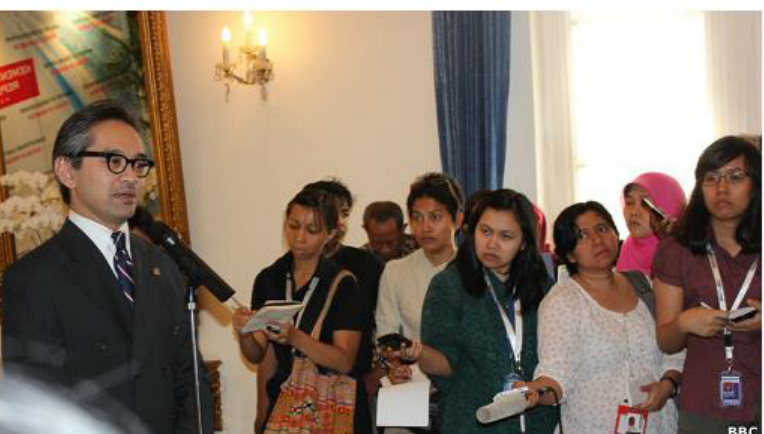
\includegraphics[width=83.58mm,height=119.39mm]{../../images/llm/page_018_img_01.png}%
\end{textblock*}

\end{document}
